
\section*{Introduction}

Seasonal influenza virus infects 5--15\% of the global population every year causing an estimated 250,000 to 500,000 deaths annually \cite{flufactsheet}.
Vaccination remains the most effective public health response available.
However, frequent viral mutation results in viruses that escape previously acquired human immunity.
The World Health Organization (WHO) selects vaccine viruses to match circulating viruses, but because the process of vaccine development and distribution requires several months to complete, accurate vaccine strain selection requires a prediction of which viruses will predominate approximately one year after vaccine viruses are selected.
Current vaccine predictions favor viruses that are distinct from prior vaccine viruses in the hemagglutinin (HA) protein, which acts as the primary target of human immunity.
The hemagglutination inhibition (HI) assay \cite{hirst1943studies} is used to measure the degree of cross-reactivity between pairs of circulating viruses.
HI assays are fundamental for vaccine strain selection, but they are laborious and low-throughput compared to genome sequencing \cite{Wood:2012ii}.
As a result, researchers have developed computational methods to predict influenza fitness from sequence data alone \cite{Luksza:2014hj,Steinbruck:2014kq,Neher:2014eu}.

Despite the promise of these sequence-only models, they explicitly omit experimental measurements of antigenic or functional phenotypes.
Recent developments in computational methods and influenza virology have made it feasible to integrate these important metrics of influenza fitness into a single predictive model.
For example, phenotypic measurements of antigenic drift are now accessible through phylogenetic models \cite{Neher:2016hy} and functional phenotypes for HA are available from deep mutational scanning experiments \cite{Lee2018}.
We describe an approach to integrate previously disparate sequence-only models of influenza evolution with high-quality experimental measurements of antigenic drift and functional constraint.

\textit{Brief summary of model implementation here including reference to Fig.~\ref{fig:model}.}

\section*{Results}

\subsection*{Models accurately forecast evolution of simulated populations of {A/H3N2-like viruses}}

The long-term evolution of influenza A/H3N2 hemagglutinin has been previously described as a balance between positive selection for substitutions at epitopes that enable escape from adaptive immunity and purifying selection on domains required to maintain the protein's primary functions of binding and membrane fusion \cite{Bush:1999vj,Neher2013,Luksza:2014hj,Koelle:2015dh}.
To test the ability of our models to accurately detect these evolutionary patterns under controlled conditions, we first simulated the long-term evolution of five independent populations of A/H3N2-like viruses for 5,000 generations each using SANTA-SIM \cite{Jariani2019}.
We seeded each simulated population with the full length HA from A/Beijing/32/1992 such that all simulated sequences contained signal peptide, HA1, and HA2 domains.
We defined purifying selection across all three domains, allowing the preferred amino acid at each site to change at a fixed rate over time.
We additionally defined exposure-dependent selection for 129 putative epitope sites in HA1 \cite{Wolf:2006da} to impose an effect of cross-immunity that would allow mutations at those sites to increase viral fitness despite underlying purifying selection.
These selective constraints produced phylogenetic structures and accumulation of epitope and non-epitope mutations that were consistent with phylogenies of natural A/H3N2 HA (Supplemental Figure \ref{sup_fig:simulated_h3n2_ha_phylogeny}).

Under the evolutionary constraints of our simulations, we expected the models to learn positive coefficients for cross-immunity and negative coefficients for non-epitope mutations corresponding to the fitness benefits of novel epitope sequences and costs of accumulating deleterious mutations.
We reasoned that because LBI and delta frequency measure the recent success of samples without any mechanistic explanation for that success, these two models should be assigned positive coefficients and should outperform the individual mutation models by being able to simultaneously represent benefits of epitope mutations and costs of non-epitope mutations with a single metric.
To achieve the same accuracy from mutation-only models, we anticipated that these two models would need to be combined.
To test these hypotheses, we trained models for each individual fitness metric on 20 years of simulated sequences corresponding to generations 1000--3000 where 100 generations represents one year.
As a positive control, we trained a model on the true fitness of each sample as measured by the simulator.
To control for variability in distances between seasons, we evaluated all models relative to the observed distance between seasons (the adjusted distance between seasons).
This distance corresponded to a model without an exponential growth parameter which we labeled as the ``naive'' model.

The average distance per year between populations averaged 18 +/- 5 amino acids in the naive model (Supplemental Fig.~\ref{sup_fig:weighted_distance_between_timepoints}).
On average, all models reduced this distance with LBI performing the best by reducing this distance to the future by over four amino acids (Fig.~\ref{fig:model_accuracy_and_coefficients_for_simulated_populations}).
As expected, the true fitness metric always outperformed the naive model.
The non-epitope metric also consistently outperformed the naive model, predicting the future nearly as well as the true fitness.
Surprisingly, cross-immunity did not accurately forecast future populations, receiving instead an average coefficient near zero in most training windows.
While the delta frequency metric was not as accurate as LBI, it was considerably less variable with an average adjusted distance similar to the non-epitope metric.
Interestingly, the coefficients for non-epitope mutations, LBI, and delta frequency were stably non-zero across all training windows with standard deviations ranging from 0.16 to 0.42.
In contrast, the true fitness metric's coefficients gradually varied more over time with a standard deviation of 0.62.

\begin{figure*}[t]
  \begin{center}
  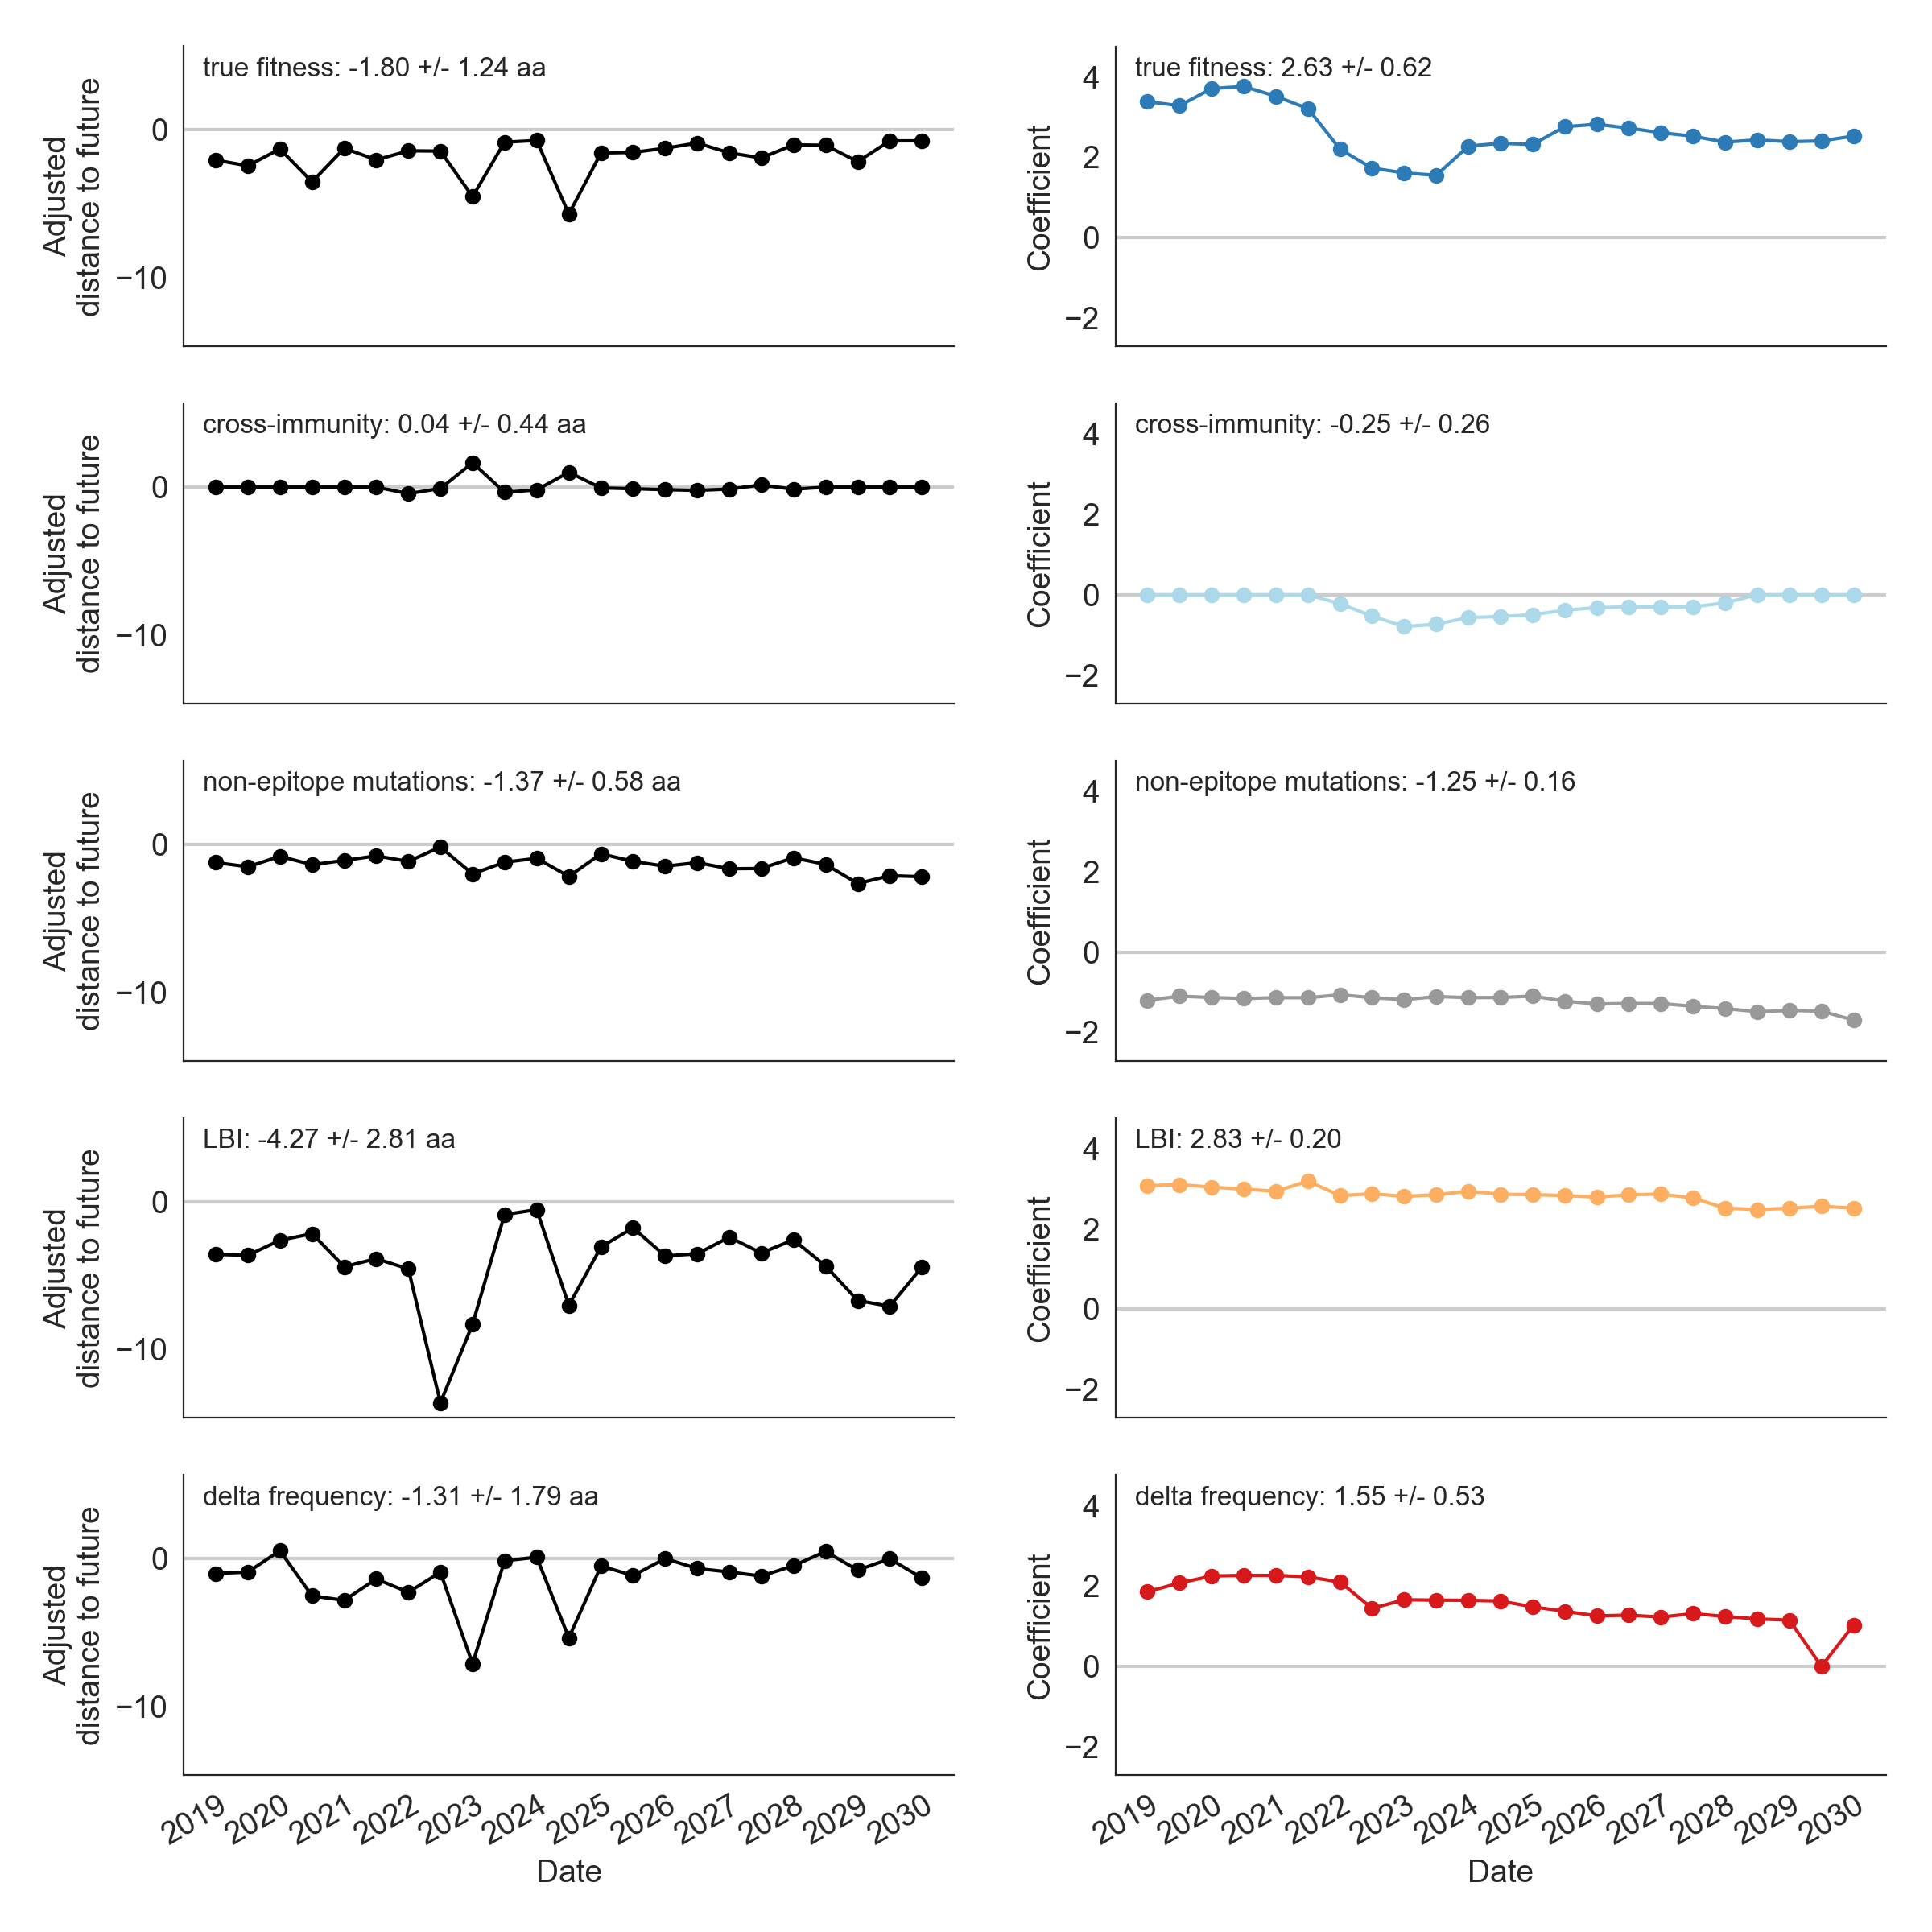
\includegraphics[width=\textwidth]{figures/model-accuracy-and-coefficients-for-simulated-populations.png}
  \caption{Model a) accuracy and b) coefficients for simulated populations of A/H3N2-like viruses.}
  \label{fig:model_accuracy_and_coefficients_for_simulated_populations}
  \end{center}
\end{figure*}

We tested our hypothesis that composite models of cross-immunity and non-epitope mutations would perform as well as LBI or delta frequency.
We further tested the relationship between LBI and these two individual metrics by fitting composite models with all combinations of these three predictors.
Surprisingly, cross-immunity provided no additional accuracy to the non-epitope metric, while neither of these mutation-based metrics provided any improvement over LBI (Supplemental Fig.~\ref{sup_fig:composite_model_accuracy_and_coefficients_for_simulated_populations}).
In the latter models, LBI maintained a consistent coefficient across all training windows while the models assigned both cross-immunity and non-epitope metrics coefficients near zero.
These results suggest that non-epitope mutations and LBI are mutually exclusive and either metric is sufficient to forecast the evolution of these simulated populations.

\textit{Repeat simulations with multiple epochs to show model coefficients can reflect these underlying changes to evolutionary constraints.}

\subsection*{Models based on X metrics most accurately forecast natural populations of A/H3N2 viruses}

\subsection*{Model accuracy and coefficients reflect historical patterns of A/H3N2 evolution}

\subsection*{Composite models outperform models with individual fitness metrics}

\subsection*{Models enable selection of vaccine candidate strains}

\subsection*{Forecasts predict the rise of 3c3.A and A1b clades in February 2020}

\section*{Discussion}

\section*{Methods}

\subsection*{Simulation of influenza A/H3N2-like populations}

\subsection*{Strain selection for natural populations}

For model training and validation, we selected XX HA sequences of length >=1,700 nucleotides that were sampled between October 1994 and October 2015.
To account for known variation in sequence availability by region, we subsampled the selected sequences to a representative set of 10 viruses per month with even sampling across 10 global regions including Africa, Europe, North America, China, South Asia, Japan and Korea, Oceania, South America, Southeast Asia, and West Asia.
We excluded all samples with ambiguous year, month, and day annotations and prioritized samples with more available HI titer measurements.

For model testing, we extended the set of training and validation sequences to include HA sequences that were sampled between October 2015 and April 2019.
We used these test sequences to evaluate the out-of-sample error of fixed model parameters learned during training and validation.

\subsection*{Phylogenetic interference}

For each timepoint in model training, validation, and testing, we selected the subsampled HA sequences with collection dates up to that timepoint.
We aligned sequences with the augur align command \cite{Hadfield2018} and MAFFT v7.407 \cite{Katoh2002}.
We inferred initial phylogenies for HA sequences at each timepoint with IQ-TREE v1.6.10 \cite{Nguyen2014}.
To reconstruct time-resolved phylogenies, we applied TreeTime v0.5.6 \cite{Sagulenko2018} with the augur refine command.

\subsection*{Frequency estimation}

To account for uncertainty in collection date and sampling error, we applied a kernel density estimation (KDE) approach to calculate global sample frequencies.
Specifically, we constructed a Gaussian kernel for each sample with the mean at the reported collection date and a variance of one month, roughly corresponding to the average lag time between sample collection and submission to the GISAID database.
We estimated the frequency of each sample at each timepoint by calculating the cumulative density function of each KDE between the current and previous timepoint and normalizing the resulting values to sum to one.
We implemented this logic in the augur frequencies command.

\subsection*{Model fitting and evaluation}

\subsubsection*{Fitness model}

As in \cite{Luksza:2014hj}, we assumed that influenza A/H3N2 populations can be described by an exponential growth model.
Under this model, we estimated the future frequency of the global population, $\hat{X}$, at some time in the future, $t + \Delta{t}$, based on the current frequency, $x_{i}(t)$, and fitness, $f_{i}(t)$, of each sample $i$ as follows where the resulting future frequencies were normalized to one by $\frac{1}{Z(t)}$.

$$
\hat{X}(t + \Delta{t}) = \frac{1}{Z(t)}\sum_{i}x_{i}(t)\exp(f_{i}(t))
$$

We defined the fitness of each sample at time $t$ as the additive combination of one or more fitness metrics, $f_{i,m}$, scaled by fitness coefficients, $\beta_{m}$.

\subsubsection*{Model target}

For a model based on any given combination of fitness metrics, we found the fitness coefficients that minimized the mean weighted Hamming distance between the estimated and observed future populations as defined by,

$$
\Delta(X(t + \Delta{t}), \hat{X}(t + \Delta{t})) = \frac{(\sum_{i}x_{i}\exp(f_{i}(t))(\sum_{j}x_{j}d_{i,j})) - (\sum_{j}x_{j}(\sum_{j'}x_{j'}d_{j,j'}))}{(\sum_{i}x_{i}(\sum_{j}x_{j}d_{i,j}))},
$$

where the first term in the numerator measures the mean distance between estimated and observed populations, the second term accounts for the diversity of the future population, and the denominator accounts for the diversity between the current and future populations.
When the sequence diversity of the estimated and observed future populations are equal, the metric evaluates to zero.
When the estimated sequence diversity is closer to the center of the future population's observed diversity, the metric evaluates to a negative proportion.
We applied the Nelder-Mead minimization algorithm as implemented in SciPy \cite{SciPy} to learn fitness coefficients that minimize the average of this distance metric over all timepoints in a given training window.

\subsubsection*{Time-series cross-validation}

To obtain unbiased estimates for the out-of-sample errors of our models, we adopted the standard cross-validation strategy of training, validation, and testing.
We divided our available data into an initial training and validation set spanning October 1994 to October 2015 and an additional testing set spanning October 2015 to April 2019.
We partitioned our training and validation data into six month seasons corresponding to winter in the Northern Hemisphere (October--April) and the Southern Hemisphere (April--October) and trained models to estimate frequencies of populations one year into the future from each season in six-year sliding windows.
To calculate validation error for each training window, we applied the resulting model coefficients to estimate the future frequencies for the year after the last timepoint in the training window.
These validation errors informed our tuning of hyperparameters including a L1 regularization of the fitness coefficients, the LBI neighborhood parameter $\tau$, and the length of the training window itself.
Finally, we fixed the coefficients for each model at the mean values across all training windows and applied these fixed models to the test data to estimate the true forecasting accuracy of each model on previously unobserved data.

\subsection*{Fitness metrics}

\subsubsection*{Antigenic drift}

\subsubsection*{Functional constraint}

\subsubsection*{Clade growth}
